\documentclass[12pt,a4paper,oneside]{report}

% XeLaTeX/LuaLaTeX is recommended for exact Times New Roman and Vietnamese text.
% pdfLaTeX fallback is included to avoid engine-related compile failures.
\usepackage[a4paper,right=3cm,left=2cm,top=2cm,bottom=2cm]{geometry}
\usepackage{iftex}
\ifPDFTeX
    \usepackage[utf8]{inputenc}
    \usepackage[T5]{fontenc}
    \usepackage{mathptmx}
\else
    \usepackage{fontspec}
    \IfFontExistsTF{Times New Roman}{\setmainfont{Times New Roman}}{\setmainfont{TeX Gyre Termes}}
    \IfFontExistsTF{Consolas}{\setmonofont{Consolas}[Scale=MatchLowercase]}{\setmonofont{Latin Modern Mono}[Scale=MatchLowercase]}
\fi

\usepackage{setspace}
\singlespacing
\usepackage{indentfirst}
\setlength{\parindent}{1.27cm}
\setlength{\parskip}{0pt}

\usepackage{graphicx}
\graphicspath{{assets/images/}{assets/logos/}}
\usepackage{eso-pic}
\usepackage{float}
\usepackage{booktabs}
\usepackage{longtable}
\usepackage{array}
\usepackage{multirow}
\usepackage{caption}
\usepackage{subcaption}
\usepackage{xcolor}
\usepackage{listings}
\usepackage{enumitem}
\usepackage{titlesec}
\usepackage{tocloft}
\usepackage{fancyhdr}
\usepackage{xurl}
\usepackage{hyperref}
\usepackage[backend=biber,style=numeric,sorting=none]{biblatex}

\addbibresource{bib/references.bib}

\hypersetup{
    colorlinks=true,
    linkcolor=black,
    citecolor=black,
    urlcolor=blue,
    pdfauthor={Group 02},
    pdftitle={Vietnamese Sign Language Online Education System}
}

\definecolor{codebackground}{RGB}{248,248,248}
\definecolor{codeborder}{RGB}{215,215,215}
\definecolor{codekeyword}{RGB}{0,75,135}
\definecolor{codecomment}{RGB}{90,120,90}
\definecolor{codestring}{RGB}{150,70,30}

\lstdefinestyle{sqlstyle}{
    language=SQL,
    basicstyle=\ttfamily\small,
    keywordstyle=\color{codekeyword}\bfseries,
    commentstyle=\color{codecomment}\itshape,
    stringstyle=\color{codestring},
    backgroundcolor=\color{codebackground},
    frame=single,
    rulecolor=\color{codeborder},
    breaklines=true,
    breakatwhitespace=false,
    columns=fullflexible,
    keepspaces=true,
    showstringspaces=false,
    numbers=left,
    numberstyle=\tiny\color{gray},
    stepnumber=1,
    numbersep=8pt,
    xleftmargin=1.5em,
    framexleftmargin=1.2em,
    captionpos=b,
    tabsize=4
}

\lstdefinestyle{terminalstyle}{
    basicstyle=\ttfamily\small,
    backgroundcolor=\color{codebackground},
    frame=single,
    rulecolor=\color{codeborder},
    breaklines=true,
    columns=fullflexible,
    keepspaces=true,
    showstringspaces=false,
    numbers=left,
    numberstyle=\tiny\color{gray},
    numbersep=8pt,
    xleftmargin=1.5em,
    framexleftmargin=1.2em,
    captionpos=b
}

\lstnewenvironment{sqlcode}[1][]{\lstset{style=sqlstyle,#1}}{}
\lstnewenvironment{terminalcode}[1][]{\lstset{style=terminalstyle,#1}}{}
\renewcommand{\lstlistingname}{Code Listing}
\renewcommand{\lstlistlistingname}{List of Code Listings}

\captionsetup{font=small,labelfont=bf,labelsep=period}
\renewcommand{\arraystretch}{1.2}
\setlength{\emergencystretch}{2em}
\setlist{nosep,leftmargin=1.2cm}

\titleformat{\chapter}[display]
    {\normalfont\bfseries\centering\Large}
    {CHAPTER \thechapter}
    {0.5em}
    {\MakeUppercase}
\titlespacing*{\chapter}{0pt}{-10pt}{20pt}

\titleformat{\section}
    {\normalfont\bfseries\large}
    {\thesection}
    {0.75em}
    {}
\titleformat{\subsection}
    {\normalfont\bfseries\normalsize}
    {\thesubsection}
    {0.75em}
    {}

\pagestyle{fancy}
\fancyhf{}
\fancyhead[L]{Vietnamese Sign Language Online Education System}
\fancyhead[R]{Group 02}
\fancyfoot[C]{\thepage}
\renewcommand{\headrulewidth}{0.4pt}
\renewcommand{\footrulewidth}{0pt}

\newcommand{\coverborder}{%
    \AddToShipoutPictureBG*{%
        \AtPageLowerLeft{%
            
\includegraphics[width=\paperwidth,height=\paperheight]{\detokenize{assets/logos/khung-vien-trang-bia-Word-10.jpg}}%
        }%
    }%
}

\begin{document}

\begin{titlepage}
    \coverborder
    \thispagestyle{empty}
    \centering
    {\bfseries\Large HỌC VIỆN CÔNG NGHỆ BƯU CHÍNH VIỄN THÔNG\par}
    \vspace{0.35cm}
    {\bfseries\large KHOA CÔNG NGHỆ THÔNG TIN 1\par}
    \vspace{1.1cm}

    \IfFileExists{assets/logos/logo_ptit.jpg}{
        
\includegraphics[height=3.2cm,keepaspectratio]{assets/logos/logo_ptit.jpg}
    }{
        \fbox{\parbox[c][3.0cm][c]{3.0cm}{\centering PTIT\\Logo}}
    }

    \vspace{1.2cm}
    {\bfseries\Large MAJOR ASSIGNMENT REPORT\par}
    \vspace{0.4cm}
    {\bfseries\Large DATABASE MANAGEMENT SYSTEMS\par}
    \vspace{1.2cm}

    {\bfseries\large ĐỀ TÀI:\par}
    \vspace{0.3cm}
    {\bfseries\Large HỆ THỐNG GIÁO DỤC TRỰC TUYẾN NGÔN NGỮ KÝ HIỆU VIỆT NAM\par}
    \vspace{0.25cm}
    {\itshape\large Vietnamese Sign Language Online Education System\par}

    \vfill

    \begin{center}
        \begin{tabular}{>{\bfseries}p{4cm}p{9cm}}
            Class: & D23CQCE06-B \\
            Group: & 02 \\
            Course: & Hệ quản trị cơ sở dữ liệu \\
        \end{tabular}
    \end{center}

    \vspace{0.3cm}
    \begin{center}
        \begin{tabular}{>{\bfseries}p{1cm}p{7cm}p{4cm}}
            No. & Student name & Student ID \\
            \midrule
            1 & Vũ Đình Hiếu & B23DCCE036 \\
            2 & Đặng Văn Chiến & B23DCCE012 \\
            3 & Bùi Quang Thắng & B23DCCN751 \\
        \end{tabular}
    \end{center}

    \vfill
    {\bfseries Hà Nội, \the\year\par}
\end{titlepage}

\pagenumbering{roman}
\setcounter{page}{1}

\chapter*{Acknowledgements}
\addcontentsline{toc}{chapter}{Acknowledgements}
This section will be completed in the final version of the report.

\chapter*{Abstract}
\addcontentsline{toc}{chapter}{Abstract}
This section will summarize the objectives, database design, implementation scope, and key outcomes of the project.

\tableofcontents
\clearpage
\phantomsection
\addcontentsline{toc}{chapter}{List of Figures}
\listoffigures
\clearpage
\phantomsection
\addcontentsline{toc}{chapter}{List of Tables}
\listoftables
\clearpage
\phantomsection
\addcontentsline{toc}{chapter}{List of Code Listings}
\lstlistoflistings
\clearpage
\chapter*{List of Abbreviations}
\addcontentsline{toc}{chapter}{List of Abbreviations}

\begin{longtable}{p{3cm}p{11cm}}
\toprule
\textbf{Abbreviation} & \textbf{Meaning} \\
\midrule
DBMS & Database Management System \\
DDL & Data Definition Language \\
DML & Data Manipulation Language \\
ERD & Entity Relationship Diagram \\
FK & Foreign Key \\
PK & Primary Key \\
RLS & Row-Level Security \\
SQL & Structured Query Language \\
UUID & Universally Unique Identifier \\
VSL & Vietnamese Sign Language \\
\bottomrule
\end{longtable}

\clearpage

\pagenumbering{arabic}
\setcounter{page}{1}

\chapter{Problem Introduction}
\label{chap:problem-introduction}

\section{Problem Statement}
Learning Vietnamese Sign Language (VSL) remains a challenge because existing learning resources are often fragmented across videos, social media posts, classroom notes, and small independent websites. In practice, learners usually do not have access to a centralized platform where they can search vocabulary, follow structured learning paths, enroll in courses, monitor their progress, and maintain long-term motivation. This also creates difficulties for teachers and administrators who need to manage educational content and learner activity in a consistent and systematic way.

The educational problem is therefore not only about delivering content, but also about organizing learning data in a way that supports real teaching and learning workflows. A dedicated online platform for Vietnamese sign language requires an integrated database capable of handling users, roles, vocabulary resources, courses, lessons, enrollments, progress records, feedback, notifications, and learner engagement data. Without such a database foundation, the platform would face problems of redundancy, inconsistency, and poor maintainability.

To address this need, the project develops a database system for an online Vietnamese sign language learning platform. The system is intended not only to store information, but also to support practical educational processes such as student enrollment, progress updates, streak tracking, notifications, reporting, and interaction through a database demo application.

\begin{figure}[htbp]
    \centering
    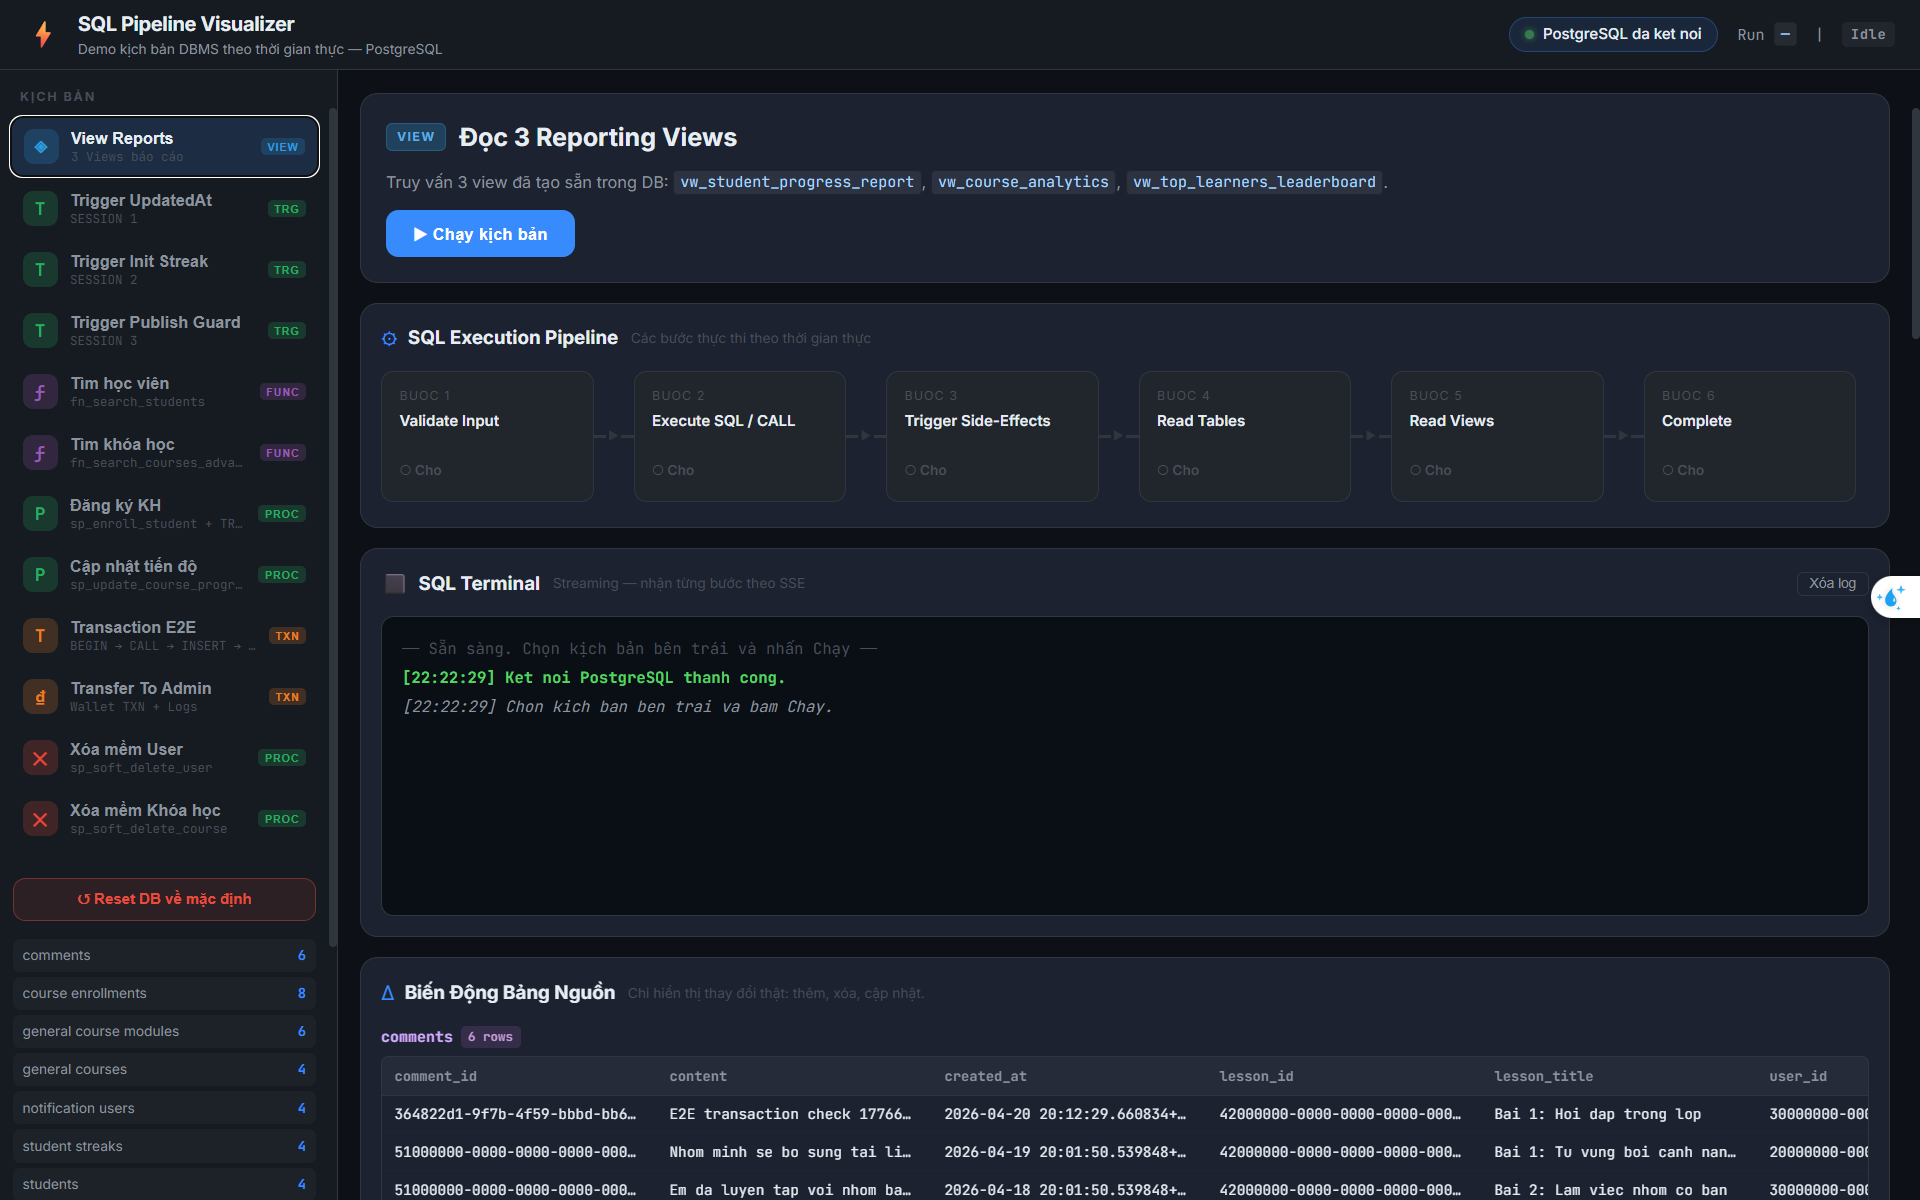
\includegraphics[width=0.9\textwidth]{assets/images/figure_1_1}
    \caption{Problem context and motivation for building the Vietnamese sign language learning platform.}
    \label{fig:introduction-context}
\end{figure}

\section{Project Objectives}
The main objective of this project is to design and implement a reliable database foundation for an online Vietnamese sign language learning platform. The database must support the storage, retrieval, and controlled processing of information related to learners, teachers, courses, lessons, dictionary content, and learning activities.

From a database perspective, the project is expected to organize data clearly, maintain consistency, support access control, and provide a stable basis for learning-related operations. More specifically, the project aims to:
\begin{itemize}
    \item design a normalized relational schema that clearly represents the key entities and relationships of the system;
    \item ensure data consistency through primary keys, foreign keys, unique constraints, check constraints, and transaction control;
    \item implement database-side business logic using views, functions, procedures, and triggers;
    \item support role-based access patterns for administrators, teachers, and students;
    \item provide data structures for enrollments, progress tracking, comments, notifications, and engagement features;
    \item prepare the database for integration with a web-based demo application that illustrates major workflows.
\end{itemize}

\section{Scope and Limitations}
The scope of the project focuses on the database layer of the platform. It includes the design and implementation of modules for user management, authentication sessions, sign language dictionary content, course organization, lesson materials, student enrollments, learning progress, comments, microlearning, gamification, notifications, and transaction logging. The project also covers database mechanisms such as views, functions, procedures, triggers, soft delete, and transaction handling for important business scenarios.

However, the current implementation also has clear limitations. First, the project focuses mainly on database design and backend processing rather than full-scale production deployment. Second, advanced multimedia and intelligent features such as sign recognition, automatic interpretation, or AI-based translation are outside the current scope. Third, performance benchmarking, large-scale concurrency testing, and production-grade infrastructure evaluation are limited, because the project is mainly intended for academic demonstration and database system practice.

\begin{figure}[htbp]
    \centering
    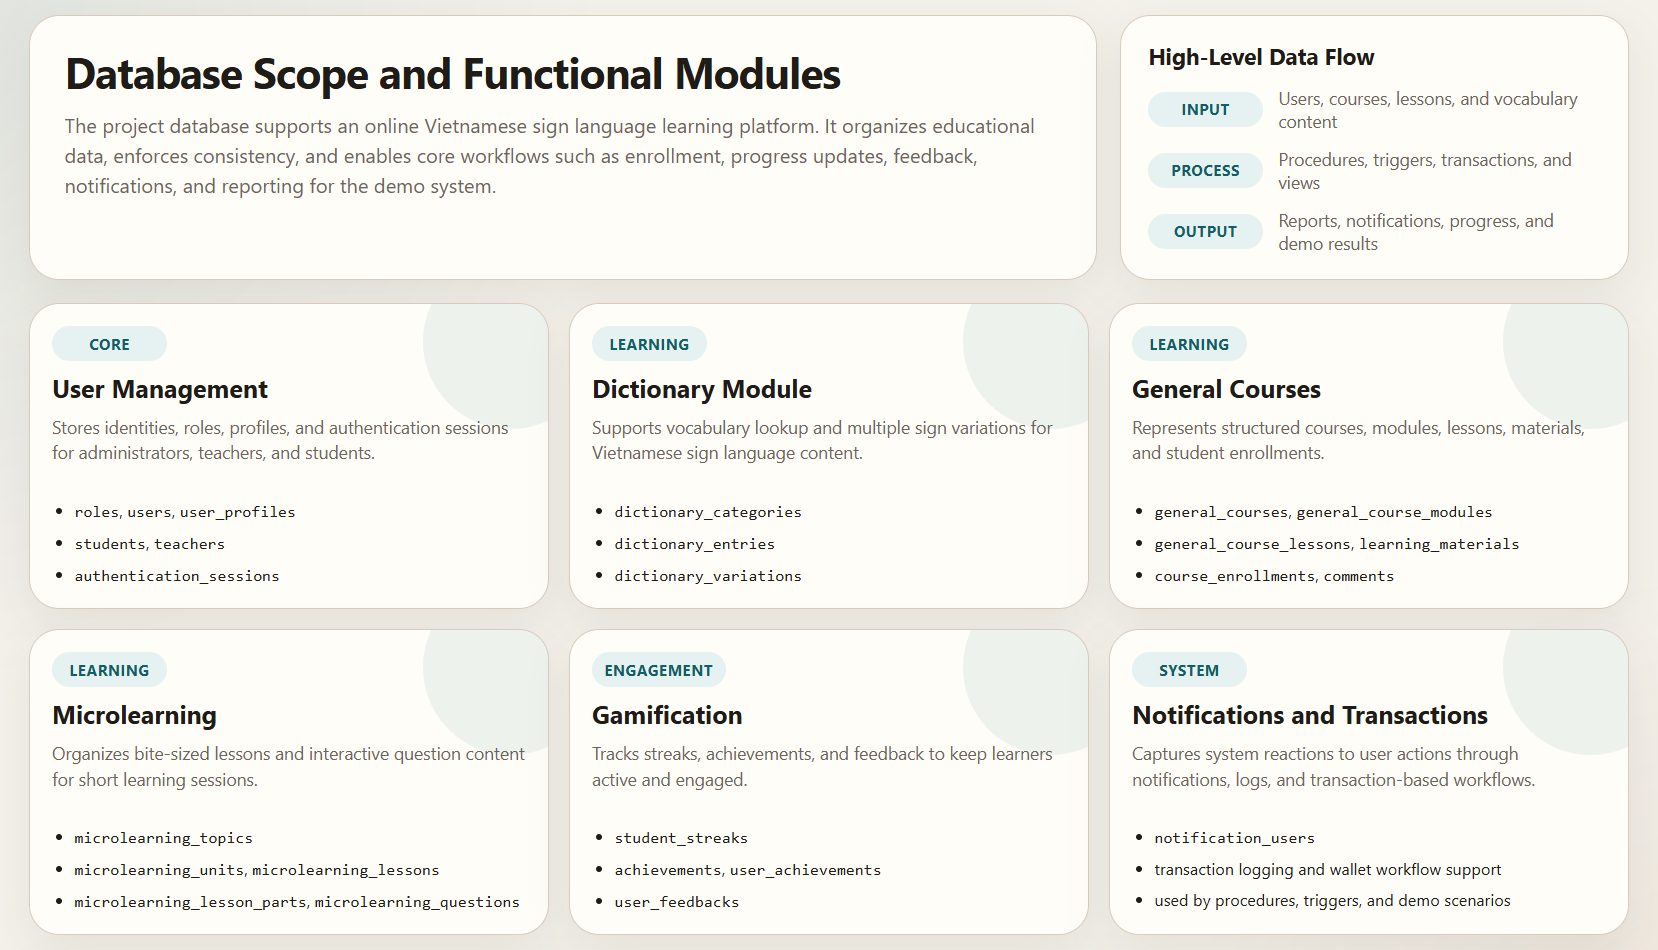
\includegraphics[width=0.9\textwidth]{assets/images/figure_1_2}
    \caption{Scope of the database system and major functional modules.}
    \label{fig:introduction-overview}
\end{figure}

\section{Report Structure}
This report is organized into several chapters that follow the development process of the project. Chapter~1 introduces the problem context, project objectives, scope, limitations, and general motivation of the study. Chapter~2 presents the configuration process, tools, technologies, and platforms used during development. Chapter~3 focuses on database design, including the entity--relationship model, schema organization, constraints, and relationships among the main modules. Chapter~4 explains the implementation details of the database system, especially the use of views, functions, procedures, triggers, and transactions, together with the demo workflow. Chapter~5 concludes the report by summarizing the main results, limitations, and possible future improvements. In addition, the report also includes a references section and appendices for supporting technical materials such as SQL scripts.

\chapter{Configuration, Tools, and Platforms}
\label{chap:configuration-tools-platforms}

\section{Database Management System}
The project uses PostgreSQL as its target database management system. This selection is appropriate because PostgreSQL supports both conventional relational database design and the advanced features required by a DBMS-oriented academic project. In the current implementation, the schema and SQL logic rely on several PostgreSQL capabilities, including \texttt{UUID} primary keys, \texttt{JSONB} fields, \texttt{CHECK} constraints, \texttt{GENERATED ALWAYS AS IDENTITY}, \texttt{TIMESTAMPTZ}, and server-side logic implemented through functions, procedures, triggers, and transactions.

The local database environment used for development and testing was verified as PostgreSQL~18.3. This version provides a strong transactional model, expressive SQL syntax, and reliable support for integrity constraints and procedural extensions. These characteristics make PostgreSQL well suited to a project that emphasizes data consistency, business-rule enforcement, and database-side processing for workflows such as enrollment, progress tracking, notifications, and transaction logging.

% Ghi chú tiếng Việt:
% Phần này giải thích vì sao chọn PostgreSQL.
% Điểm nên nhấn mạnh là dự án không chỉ dùng bảng và truy vấn cơ bản,
% mà còn dùng nhiều tính năng nâng cao của PostgreSQL như UUID, JSONB,
% CHECK constraint, trigger, function, procedure và transaction.
% Trong máy hiện tại, phiên bản DB đã kiểm tra được là PostgreSQL 18.3.

\section{Development Environment}
The development environment combines SQL source files, a Flask-based demo application, and supporting tools for editing, testing, and database inspection. According to the repository structure, the database is initialized from \path{ERD.sql}, populated by \path{seed_data.sql}, and extended with procedural logic from \path{procedure_trigger_transaction.sql}. The demonstration layer is implemented in Python and Flask under the \path{demo/} directory, where the application connects directly to PostgreSQL and exposes the main database scenarios through a web interface.

The local machine used for development provides a Windows-based environment with Visual Studio Code for source editing, Git for version control, Python 3.14.4 for runtime execution, Flask 3.1.3 for the demo application, and PostgreSQL 18.3 for data storage and processing. For database interaction, the system also has \texttt{psql} 18.3 and pgAdmin~4 installed, which are appropriate tools for script execution, inspection, and manual verification of the database state.

\begin{figure}[htbp]
    \centering
    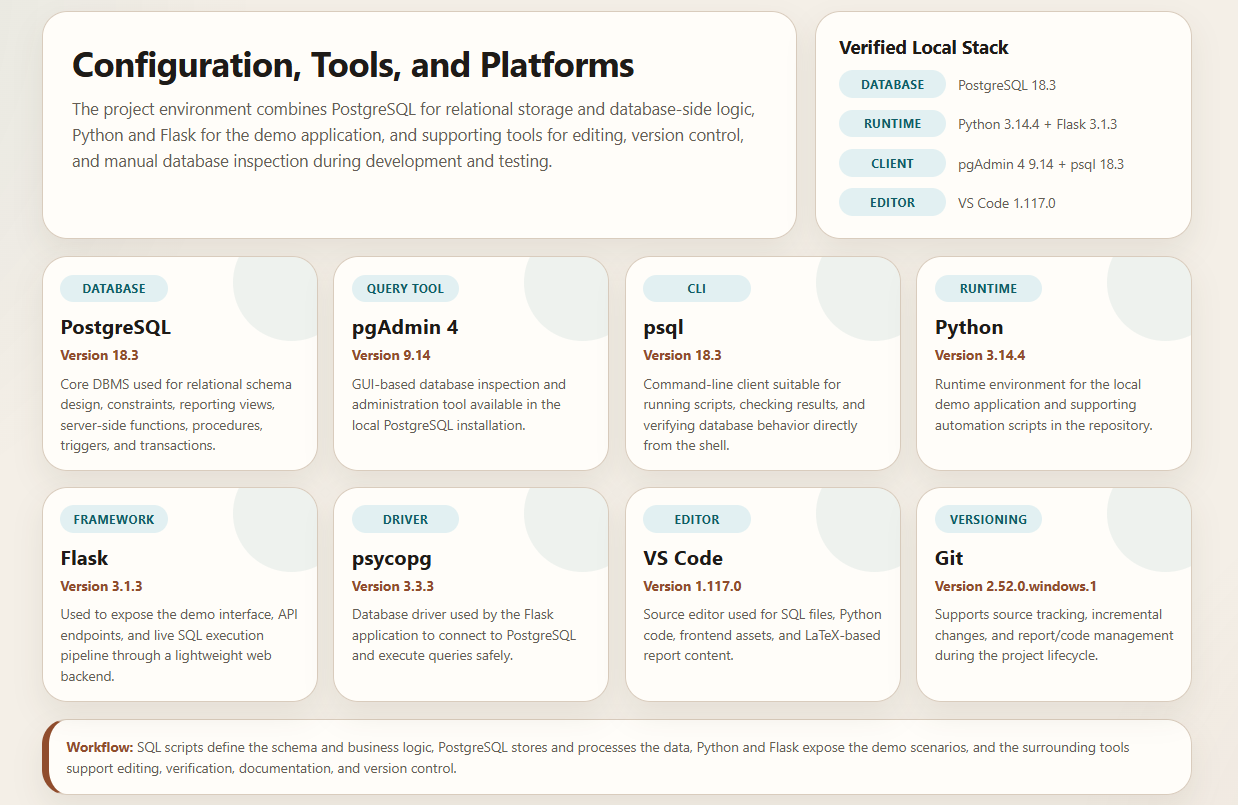
\includegraphics[width=0.96\textwidth]{assets/images/figure_2_1}
    \caption{Development stack and core tools used in the project environment.}
    \label{fig:chapter2-stack}
\end{figure}

% Ghi chú tiếng Việt:
% Phần này mô tả môi trường phát triển thực tế.
% Có thể hiểu đơn giản là:
% SQL scripts -> PostgreSQL -> Flask demo -> browser để trình diễn.
% Đồng thời nêu rõ editor, runtime, Git, và công cụ DB client đang có trên máy.
%
% Ảnh 2.1 đang dùng file figure_2_1.png.
% Nội dung ảnh nên thể hiện stack công nghệ chính của dự án:
% PostgreSQL, pgAdmin/psql, Python, Flask, Git, VS Code và các SQL scripts chính.

\section{Tools and Technologies}
\begin{table}[H]
    \centering
    \small
    \caption{Tools and technologies used in the project}
    \label{tab:tools-technologies}
    \begin{tabular}{p{3.2cm}p{4.2cm}p{6.2cm}}
        \toprule
        \textbf{Category} & \textbf{Tool/Technology} & \textbf{Purpose} \\
        \midrule
        Database & PostgreSQL 18.3 & Relational database implementation, schema definition, constraints, triggers, procedures, functions, and transactions \\
        Query Tool & pgAdmin 4 9.14 / \texttt{psql} 18.3 & Database inspection, script execution, and manual verification of tables and SQL logic \\
        Programming Language & Python 3.14.4 & Runtime environment for the Flask demo application and database connectivity scripts \\
        Web Framework & Flask 3.1.3 & Web backend for the demo interface, API endpoints, and SSE-based progress updates \\
        Database Driver & psycopg 3.3.3 & PostgreSQL connectivity layer used by the Python demo application \\
        Frontend & HTML, CSS, JavaScript & Interactive browser-based interface for demonstrating views, triggers, procedures, and transactions \\
        Source Editor & Visual Studio Code 1.117.0 & Editing SQL files, Python source code, frontend assets, and report files \\
        Documentation & LaTeX / Overleaf & Academic report preparation and final document formatting \\
        Version Control & Git 2.52.0.windows.1 & Source code management and report version tracking \\
        \bottomrule
    \end{tabular}
\end{table}

The technology stack reflects the structure of the project itself. PostgreSQL serves as the central platform for data storage and business logic, while Python and Flask connect the database layer to a demonstrable user-facing interface. The remaining tools support development workflow, editing, version control, and final documentation.

% Ghi chú tiếng Việt:
% Bảng này đã điền sẵn theo công cụ phát hiện được trên máy và trong repo.
% Nếu sau này bạn muốn rút gọn, có thể giữ các hàng quan trọng nhất:
% PostgreSQL, pgAdmin/psql, Python, Flask, Git, VS Code, LaTeX/Overleaf.
% Nếu nhóm có dùng thêm Docker, Postman hoặc draw.io thì có thể thêm một hàng mới.

\section{Hardware Configuration}
The hardware configuration used for development and testing is sufficient for a medium-scale academic database project. The local machine used for this work is equipped with a 13th Gen Intel(R) Core(TM) i5-13420H processor, 15.64~GB of physical memory, and local fixed drives totaling approximately 426.28~GB of storage capacity. At the time of inspection, the machine provided two main fixed drives: a 226.28~GB system drive and a 200.00~GB workspace drive.

The operating environment is a 64-bit Windows platform, identified locally as build 26200 with display version 25H2. This setup is adequate for running PostgreSQL, Python, Flask, the browser-based demo interface, and supporting development tools at the same time. For the scope of the project, the hardware requirements are moderate, but the available CPU, memory, and storage are sufficient for schema creation, data seeding, SQL testing, and interactive demonstration.

\begin{itemize}
    \item CPU: 13th Gen Intel(R) Core(TM) i5-13420H
    \item RAM: 15.64 GB
    \item Storage: 226.28 GB system drive + 200.00 GB workspace drive
    \item Operating System: Windows x64, display version 25H2, build 26200
\end{itemize}

\begin{figure}[htbp]
    \centering
    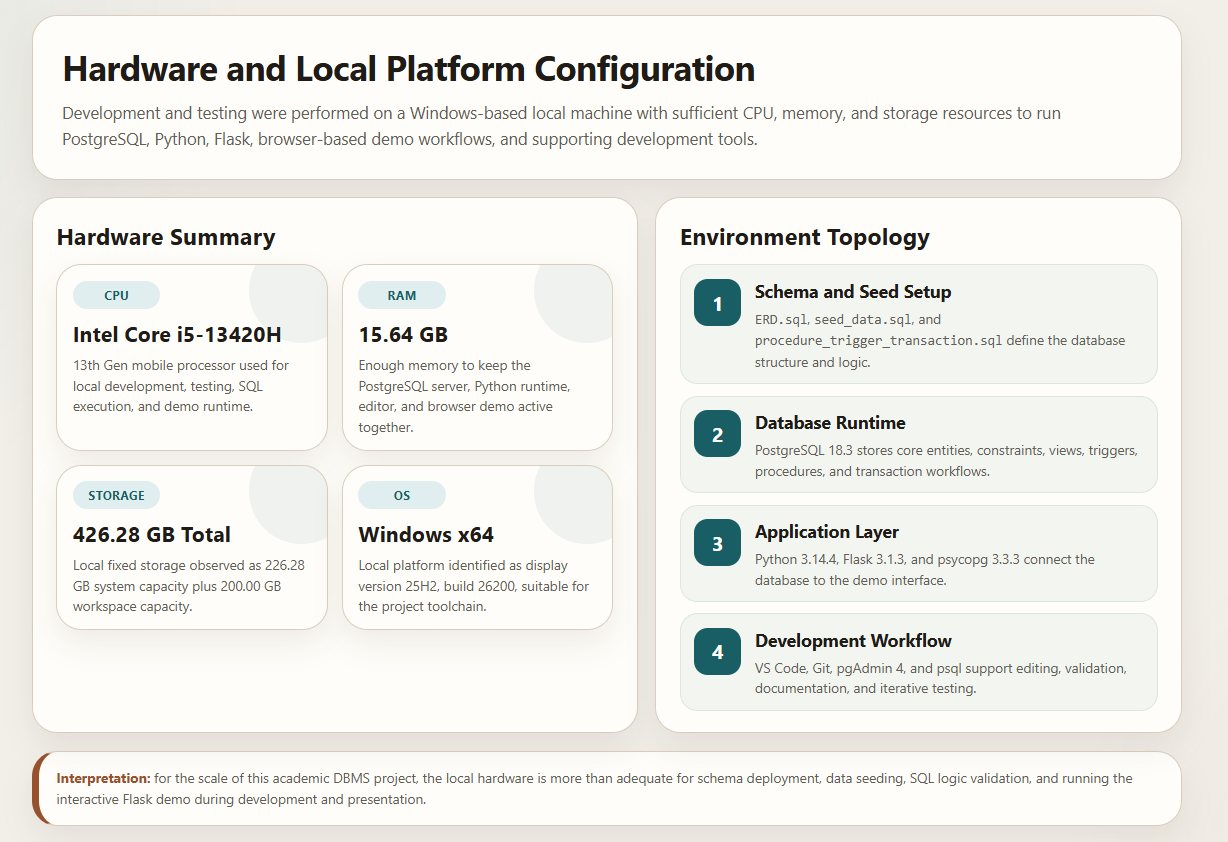
\includegraphics[width=0.96\textwidth]{assets/images/figure_2_2}
    \caption{Hardware and local platform configuration used for development and testing.}
    \label{fig:chapter2-hardware}
\end{figure}

% Ghi chú tiếng Việt:
% Phần này dùng cấu hình máy thật đã kiểm tra được trong môi trường hiện tại.
% Nếu bạn muốn trình bày ngắn hơn, chỉ cần giữ 4 dòng CPU, RAM, Storage, Operating System.
% Nếu sau này chạy demo trên một máy khác, nên sửa lại mục này cho đúng với máy đem đi bảo vệ.
%
% Ảnh 2.2 đang dùng file figure_2_2.png.
% Ảnh này nên minh họa hai ý:
% (1) cấu hình phần cứng và hệ điều hành,
% (2) cách các thành phần môi trường local phối hợp với nhau khi chạy dự án.

\chapter{Database Design Overview}

\section{System Overview}

The Vietnamese Sign Language Online Education System is designed as a relational database system that supports dictionary lookup, structured online courses, microlearning activities, user management, and learning engagement features. From a database perspective, the system must store both relatively static educational content, such as dictionary entries and course materials, and dynamic learner-generated data, such as enrollments, progress, comments, streaks, feedback, and notifications.

The database design follows a modular structure. Each module is responsible for a distinct functional area, while shared entities such as \texttt{users}, \texttt{students}, and \texttt{teachers} provide integration across the whole system. This approach improves maintainability because each group of tables has a clear responsibility, and it also supports future extension of the platform without forcing major changes to unrelated modules.

The schema uses PostgreSQL data types and constraints to improve data integrity. Universally Unique Identifiers are used for most business entities, while identity integers are used for small reference tables such as roles, categories, and achievements. Foreign key constraints define the relationships between entities, unique constraints prevent duplicated business records, and check constraints restrict invalid values such as negative progress or unsupported course statuses.

\section{Entity Relationship Diagram}

Figure~\ref{fig:erd-system} presents the Entity Relationship Diagram (ERD) of the database. The diagram shows the main base tables, their primary keys, foreign keys, and relationships. It also includes several derived reporting views at the bottom of the diagram; these views are not independent data storage tables, but are used to simplify analytical queries and report generation.

\begin{figure}[H]
    \centering
    
\includegraphics[width=\textwidth,height=0.78\textheight,keepaspectratio]{\detokenize{assets/images/ERD Diagram.png}}
    \caption{Entity Relationship Diagram of the Vietnamese Sign Language Online Education System}
    \label{fig:erd-system}
\end{figure}

The ERD shows that \texttt{users} is the central entity of the system. A user belongs to a role, may have one profile, and may be extended into either a student or teacher subtype depending on the account role. Students participate in courses through enrollments, maintain learning streaks, receive achievements, submit feedback, and receive notifications. Teachers are linked to the courses they create and manage. Educational content is separated into dictionary content, general course content, and microlearning content.

\section{Database Module Summary}

Table~\ref{tab:database-modules} summarizes the major modules of the database and their responsibilities.

\begin{table}[H]
    \centering
    \caption{Summary of database modules}
    \label{tab:database-modules}
    \small
    \begin{tabular}{p{3.2cm}p{5.4cm}p{5.4cm}}
        \toprule
        \textbf{Module} & \textbf{Main Tables} & \textbf{Responsibility} \\
        \midrule
        User Management & \path{roles}, \path{users}, \path{user_profiles}, \path{students}, \path{teachers}, \path{authentication_sessions} & Stores account identities, role information, user profiles, student and teacher subtype data, and login sessions. \\
        Dictionary & \path{dictionary_categories}, \path{dictionary_entries}, \path{dictionary_variations} & Stores Vietnamese sign language vocabulary, meanings, categories, and regional video variations. \\
        General Course & \path{general_course_categories}, \path{general_courses}, \path{general_course_modules}, \path{general_course_lessons}, \path{learning_materials}, \path{course_enrollments}, \path{comments} & Supports structured courses, hierarchical lessons, learning materials, enrollments, progress tracking, and discussion. \\
        Microlearning & \path{microlearning_topics}, \path{microlearning_units}, \path{microlearning_lessons}, \path{microlearning_lesson_parts}, \path{microlearning_questions} & Supports short learning activities and quiz-based learning content. \\
        Gamification and Engagement & \path{student_streaks}, \path{achievements}, \path{user_achievements}, \path{user_feedbacks}, \path{notification_users} & Stores learner engagement data such as streaks, achievements, feedback, and notifications. \\
        \bottomrule
    \end{tabular}
\end{table}

\section{User Management Module}

The User Management module provides the identity foundation for the whole platform. It separates general account data from role-specific data, which makes the schema more normalized and avoids storing unrelated attributes in a single user table. Figure~\ref{fig:user-management-module} shows the main user-centered relationships used by the system.

\begin{figure}[H]
    \centering
    
\includegraphics[width=0.78\textwidth,height=0.78\textheight,keepaspectratio]{\detokenize{assets/images/User Management.png}}
    \caption{User management and user-related relationship diagram}
    \label{fig:user-management-module}
\end{figure}

The \texttt{roles} table defines system-level roles such as administrator, teacher, and student. Each role has a unique \texttt{role\_name}, and the \texttt{users} table references it through \texttt{role\_id}. The foreign key uses restrictive deletion behavior so that a role cannot be removed while user accounts still depend on it. This protects the consistency of access-control logic.

The \texttt{users} table stores core authentication and account information, including username, password hash, email address, role, timestamps, and soft-deletion status. The \texttt{is\_deleted} column allows the system to deactivate a user without physically removing related historical records. This design is suitable for educational systems because learning records, comments, enrollments, and achievements may still be required for auditing or reporting.

The \texttt{user\_profiles} table stores personal information such as full name, avatar URL, phone number, and date of birth. It has a one-to-one relationship with \texttt{users}, enforced by the unique constraint on \texttt{user\_id}. Separating profile data from authentication data improves clarity and keeps sensitive login information separate from display-oriented information.

The \texttt{students} and \texttt{teachers} tables implement role-specific subtypes. A student may have attributes such as grade level and school name, while a teacher may have a biography and department. Both tables use \texttt{user\_id} as their primary key and foreign key to \texttt{users}. This pattern ensures that every student or teacher record must correspond to a valid user account.

The \texttt{authentication\_sessions} table stores active login sessions and optional OTP codes. The table includes an expiration timestamp and a check constraint to ensure that \texttt{expires\_at} is later than \texttt{created\_at}. This prevents invalid session lifetimes at the database level.

\section{Dictionary Module}

The Dictionary module stores sign language vocabulary and supports regional variation, which is important because signs may differ by region, context, or teaching standard. The design separates a dictionary word from its video representations, allowing one word to have multiple sign variations. Figure~\ref{fig:dictionary-module} illustrates this three-table structure.

\begin{figure}[H]
    \centering
    
\includegraphics[width=0.88\textwidth,height=0.38\textheight,keepaspectratio]{\detokenize{assets/images/dictionary_diagram.png}}
    \caption{Dictionary module relationship diagram}
    \label{fig:dictionary-module}
\end{figure}

The \texttt{dictionary\_categories} table classifies vocabulary into groups such as greetings, family, education, health, or daily activities. The \texttt{name} column is unique to prevent duplicated categories.

The \texttt{dictionary\_entries} table stores the main dictionary item. Each entry belongs to exactly one category and contains the word, its meaning, update timestamp, and soft-deletion flag. The unique constraint on \texttt{category\_id} and \texttt{word} ensures that the same word cannot be duplicated inside the same category. This allows the same term to appear in different semantic categories only when the design intentionally permits it.

The \texttt{dictionary\_variations} table stores video-based sign variations for each dictionary entry. It includes region, video URL, and description. The unique constraint on \texttt{entry\_id} and \texttt{video\_url} prevents the same video from being registered more than once for a dictionary entry. The relationship from \texttt{dictionary\_variations} to \texttt{dictionary\_entries} uses cascading deletion, which is appropriate because a variation has no independent meaning without its parent dictionary entry.

\section{General Course Module}

The General Course module supports structured learning content. It models courses as a hierarchy from category to course, module, lesson, and learning material. This hierarchy is suitable for long-form courses where students follow a planned learning path. Figure~\ref{fig:general-course-module} focuses on the main course-content hierarchy.

\begin{figure}[H]
    \centering
    
\includegraphics[width=0.96\textwidth,height=0.42\textheight,keepaspectratio]{\detokenize{assets/images/General Course.png}}
    \caption{General course module relationship diagram}
    \label{fig:general-course-module}
\end{figure}

The \texttt{general\_course\_categories} table groups courses by subject area or learning level. The \texttt{general\_courses} table stores course metadata such as teacher, category, title, description, visibility status, update timestamp, and soft-deletion flag. A course must reference a valid teacher through \texttt{teacher\_id}, ensuring that every course has an accountable instructor. The \texttt{visibility\_status} column is restricted to \texttt{DRAFT}, \texttt{PUBLISHED}, or \texttt{ARCHIVED}, which supports a controlled publishing workflow.

The \texttt{general\_course\_modules} table divides a course into ordered modules. The \texttt{order\_index} column must be positive, and the unique constraint on \texttt{course\_id} and \texttt{order\_index} prevents two modules in the same course from having the same position. This maintains a deterministic learning sequence.

The \texttt{general\_course\_lessons} table further divides modules into ordered lessons. It follows the same ordering strategy as modules, using a positive \texttt{order\_index} and a uniqueness rule within each module. The \texttt{learning\_materials} table stores lesson resources such as video URLs and optional transcripts in \texttt{JSONB} format. Using \texttt{JSONB} for transcripts gives flexibility for structured captions, timestamps, or sign annotations without adding many specialized columns.

The \texttt{course\_enrollments} table represents the many-to-many relationship between students and courses. Each enrollment stores progress as a percentage from 0 to 100\%, and the unique constraint on \texttt{student\_id} and \texttt{course\_id} prevents duplicate enrollment records for the same student and course. The \texttt{comments} table allows users to discuss specific lessons and provides timestamped interaction data.

\section{Microlearning Module}

The Microlearning module supports short and focused learning activities. Unlike the General Course module, which is designed for longer structured courses, microlearning content is organized into compact topics, units, lessons, lesson parts, and questions. Figure~\ref{fig:microlearning-module} shows the sequential structure of the microlearning content model.

\begin{figure}[H]
    \centering
    
\includegraphics[width=0.96\textwidth,height=0.42\textheight,keepaspectratio]{\detokenize{assets/images/microlearning_diagram.png}}
    \caption{Microlearning module relationship diagram}
    \label{fig:microlearning-module}
\end{figure}

The \texttt{microlearning\_topics} table represents broad learning themes. Each topic contains multiple \texttt{microlearning\_units}, and each unit contains multiple \texttt{microlearning\_lessons}. Both units and lessons use \texttt{order\_index} columns to preserve the intended learning sequence.

The \texttt{microlearning\_lesson\_parts} table breaks a lesson into smaller content blocks. The \texttt{part\_type} column can be used to distinguish between explanation, practice, quiz, or other activity types. Each part has a positive order index and is unique within its parent lesson.

The \texttt{microlearning\_questions} table stores quiz questions associated with lesson parts. It includes the question text, question type, answer options in \texttt{JSONB}, and the correct answer. The use of \texttt{JSONB} for \texttt{options\_json} allows the system to represent different question formats while keeping the relational structure simple.

\section{Gamification and Engagement Module}

The Gamification and Engagement module records learner motivation and communication features. These tables are not the core educational content, but they are essential for increasing student retention and supporting interaction with the platform.

The \texttt{student\_streaks} table stores each student's current streak, highest streak, and last activity date. The table enforces non-negative streak values and ensures that the highest streak is always greater than or equal to the current streak. The unique constraint on \texttt{student\_id} guarantees that each student has only one streak record.

The \texttt{achievements} table defines available achievements, including title, description, and icon URL. The \texttt{user\_achievements} table links users to achievements they have earned. Its composite primary key on \texttt{user\_id} and \texttt{achievement\_id} prevents duplicate achievement awards.

The \texttt{user\_feedbacks} table stores user ratings and textual feedback. The rating column is optional, but when provided, it must be between 1 and 5. This constraint prevents invalid feedback scores and supports reliable evaluation statistics.

The \texttt{notification\_users} table stores notifications sent to users. It includes the notification title, message, read status, and creation timestamp. This table can support system messages such as successful enrollment notifications, course publication announcements, achievement messages, or administrative alerts.

\section{Relationship and Integrity Design}

The schema uses several integrity mechanisms to reduce inconsistent data. Primary keys uniquely identify each record, while foreign keys preserve referential integrity across modules. Cascading delete is used when child records depend entirely on the parent record, such as course modules under a course or dictionary variations under a dictionary entry. Restrictive deletion is used for reference or ownership relationships where deleting a parent could damage important historical or administrative data.

Unique constraints are used for important business rules. For example, usernames and role names must be unique, each student can enroll in the same course only once, and ordered course modules cannot share the same order index inside a course. Check constraints are used to validate bounded values such as enrollment progress, feedback ratings, streak counts, and course visibility status.

Indexes are defined on frequently joined or filtered columns, especially foreign keys and soft-deletion flags. This improves query performance for common operations such as listing courses by teacher, retrieving lessons by module, finding enrollments by student, and filtering active records.

\section{Design Rationale}

The overall database design follows normalization principles while still supporting practical application requirements. User identity, profile information, educational content, progress data, and engagement data are stored in separate but connected tables. This reduces redundancy and makes the schema easier to maintain.

The use of UUID primary keys for major entities supports distributed application development and avoids exposing predictable sequential identifiers for user-facing records. Identity integer keys are still used for compact reference tables where sequential identifiers are simple and efficient.

Soft deletion is used for important entities such as users, dictionary entries, and courses. This approach supports data recovery, auditability, and historical reporting. At the same time, child records use cascading deletion where their lifecycle is strictly dependent on the parent entity.

In summary, the database schema provides a structured foundation for an online Vietnamese sign language learning platform. It supports core academic content, learner progress, dictionary lookup, microlearning, and engagement features while maintaining consistency through relational constraints and PostgreSQL-specific capabilities.

\chapter{Implementation and Deployment}

\section{Database Schema Implementation}

The database schema was implemented in PostgreSQL using Data Definition Language (DDL). The implementation focuses on correctness, normalization, referential integrity, and extensibility. The schema is divided into five functional modules: User Management, Dictionary, General Course, Microlearning, and Gamification and Engagement. Each module contains tables that represent a specific group of business entities, while foreign keys connect the modules into a consistent relational model.

The complete schema script is stored in \texttt{Scripts/TABLE.sql}. This section presents the main implementation decisions and representative DDL fragments that demonstrate how the schema was created.

\subsection{DDL Implementation Overview}

The schema uses PostgreSQL 15+ features such as UUID primary keys, identity columns, timestamp columns, JSONB fields, check constraints, unique constraints, and foreign key actions. Because several tables use \texttt{gen\_random\_uuid()}, the database should enable the \texttt{pgcrypto} extension before executing the table creation script.

\begin{sqlcode}[caption={PostgreSQL extension required for UUID generation},label={lst:ddl-pgcrypto-extension}]
CREATE EXTENSION IF NOT EXISTS pgcrypto;
\end{sqlcode}

Table~\ref{tab:schema-module-implementation} summarizes the implemented modules and their corresponding tables.

\begin{small}
\begin{longtable}{p{3.2cm}p{10.6cm}}
\caption{Implemented database modules and tables}\label{tab:schema-module-implementation}\\
\toprule
\textbf{Module} & \textbf{Implemented Tables} \\
\midrule
\endfirsthead
\toprule
\textbf{Module} & \textbf{Implemented Tables} \\
\midrule
\endhead
User Management & \path{roles}, \path{users}, \path{user_profiles}, \path{students}, \path{teachers}, \path{authentication_sessions} \\
Dictionary & \path{dictionary_categories}, \path{dictionary_entries}, \path{dictionary_variations} \\
General Course & \path{general_course_categories}, \path{general_courses}, \path{general_course_modules}, \path{general_course_lessons}, \path{learning_materials}, \path{course_enrollments}, \path{comments} \\
Microlearning & \path{microlearning_topics}, \path{microlearning_units}, \path{microlearning_lessons}, \path{microlearning_lesson_parts}, \path{microlearning_questions} \\
Gamification and Engagement & \path{student_streaks}, \path{achievements}, \path{user_achievements}, \path{user_feedbacks}, \path{notification_users} \\
\bottomrule
\end{longtable}
\end{small}

The table creation order follows dependency direction. Reference tables such as \texttt{roles}, \texttt{dictionary\_categories}, and \texttt{general\_course\_categories} are created before dependent tables. Parent entities such as \texttt{users}, \texttt{general\_courses}, and \texttt{microlearning\_topics} are also created before child entities that contain foreign keys.

\subsection{Primary Key and Identifier Design}

The schema uses two main identifier strategies. Large business entities such as users, courses, lessons, dictionary entries, enrollments, and notifications use UUID primary keys. UUIDs are suitable for application-level entities because they reduce dependence on sequential identifiers and are convenient when records may be created by different application components.

Small reference tables use integer identity columns. Examples include \texttt{roles}, \texttt{dictionary\_categories}, \texttt{general\_course\_categories}, \texttt{microlearning\_topics}, and \texttt{achievements}. This keeps reference data compact and easy to read.

\begin{sqlcode}[caption={Representative identifier definitions},label={lst:ddl-identifier-examples}]
CREATE TABLE roles (
    role_id INTEGER GENERATED ALWAYS AS IDENTITY PRIMARY KEY,
    role_name VARCHAR(50) NOT NULL UNIQUE
);

CREATE TABLE users (
    user_id UUID PRIMARY KEY DEFAULT gen_random_uuid(),
    username VARCHAR(50) NOT NULL UNIQUE,
    password_hash VARCHAR(255) NOT NULL,
    email VARCHAR(100) UNIQUE,
    role_id INTEGER NOT NULL,
    created_at TIMESTAMPTZ NOT NULL DEFAULT CURRENT_TIMESTAMP,
    updated_at TIMESTAMPTZ NOT NULL DEFAULT CURRENT_TIMESTAMP,
    is_deleted BOOLEAN NOT NULL DEFAULT FALSE,
    CONSTRAINT fk_users_role
        FOREIGN KEY (role_id)
        REFERENCES roles (role_id)
        ON DELETE RESTRICT
);
\end{sqlcode}

The \texttt{users} table illustrates several schema design decisions. The username is mandatory and unique, while email is also unique when provided. The password is stored as a hash rather than plain text. The \texttt{created\_at} and \texttt{updated\_at} columns support auditability, and \texttt{is\_deleted} supports soft deletion.

\subsection{Referential Integrity Design}

Foreign key constraints are used throughout the schema to ensure that dependent data cannot reference non-existent parent records. The schema uses both \texttt{ON DELETE CASCADE} and \texttt{ON DELETE RESTRICT}, depending on the business meaning of each relationship.

Cascading deletion is used when a child record has no independent meaning without its parent. For example, a user profile depends on a user, course modules depend on a course, and microlearning lessons depend on a microlearning unit. Restrictive deletion is used when deleting a parent record could damage historical or administrative consistency. For example, roles and teachers are protected from deletion while user accounts or courses still reference them.

\begin{sqlcode}[caption={Representative foreign key relationships},label={lst:ddl-foreign-key-examples}]
CREATE TABLE user_profiles (
    profile_id UUID PRIMARY KEY DEFAULT gen_random_uuid(),
    user_id UUID NOT NULL UNIQUE,
    full_name VARCHAR(100) NOT NULL,
    avatar_url VARCHAR(255),
    phone_number VARCHAR(20),
    date_of_birth DATE,
    CONSTRAINT fk_user_profiles_user
        FOREIGN KEY (user_id)
        REFERENCES users (user_id)
        ON DELETE CASCADE
);

CREATE TABLE general_courses (
    course_id UUID PRIMARY KEY DEFAULT gen_random_uuid(),
    teacher_id UUID NOT NULL,
    category_id INTEGER NOT NULL,
    title VARCHAR(255) NOT NULL,
    description TEXT,
    visibility_status VARCHAR(20) NOT NULL DEFAULT 'DRAFT',
    updated_at TIMESTAMPTZ NOT NULL DEFAULT CURRENT_TIMESTAMP,
    is_deleted BOOLEAN NOT NULL DEFAULT FALSE,
    CONSTRAINT ck_course_visibility CHECK (
        visibility_status IN ('DRAFT', 'PUBLISHED', 'ARCHIVED')
    ),
    CONSTRAINT fk_courses_teacher
        FOREIGN KEY (teacher_id)
        REFERENCES teachers (user_id)
        ON DELETE RESTRICT,
    CONSTRAINT fk_courses_category
        FOREIGN KEY (category_id)
        REFERENCES general_course_categories (category_id)
        ON DELETE RESTRICT
);
\end{sqlcode}

\subsection{Business Constraints}

The DDL implementation defines database-level constraints for important business rules. These constraints reduce invalid data before it enters the system and provide a safety layer independent of application code.

\begin{small}
\begin{longtable}{p{3.4cm}p{4.8cm}p{5.8cm}}
\caption{Representative database constraints}\label{tab:ddl-business-constraints}\\
\toprule
\textbf{Constraint Type} & \textbf{Example} & \textbf{Purpose} \\
\midrule
\endfirsthead
\toprule
\textbf{Constraint Type} & \textbf{Example} & \textbf{Purpose} \\
\midrule
\endhead
Unique constraint & \path{uq_student_course_enrollment} & Prevents a student from enrolling in the same course more than once. \\
Check constraint & \path{ck_enrollment_progress} & Ensures that course progress remains between 0 and 100. \\
Check constraint & \path{ck_course_visibility} & Restricts course status to \texttt{DRAFT}, \texttt{PUBLISHED}, or \texttt{ARCHIVED}. \\
Check constraint & \path{ck_feedback_rating} & Ensures feedback ratings are between 1 and 5 when provided. \\
Unique constraint & \path{uq_module_order_per_course} & Prevents duplicate module order positions inside the same course. \\
\bottomrule
\end{longtable}
\end{small}

\begin{sqlcode}[caption={Representative business constraints},label={lst:ddl-business-constraint-examples}]
CREATE TABLE course_enrollments (
    enrollment_id UUID PRIMARY KEY DEFAULT gen_random_uuid(),
    student_id UUID NOT NULL,
    course_id UUID NOT NULL,
    progress NUMERIC(5, 2) NOT NULL DEFAULT 0.00,
    enrolled_at TIMESTAMPTZ NOT NULL DEFAULT CURRENT_TIMESTAMP,
    CONSTRAINT uq_student_course_enrollment
        UNIQUE (student_id, course_id),
    CONSTRAINT ck_enrollment_progress
        CHECK (progress >= 0 AND progress <= 100),
    CONSTRAINT fk_enrollments_student
        FOREIGN KEY (student_id)
        REFERENCES students (user_id)
        ON DELETE CASCADE,
    CONSTRAINT fk_enrollments_course
        FOREIGN KEY (course_id)
        REFERENCES general_courses (course_id)
        ON DELETE CASCADE
);

CREATE TABLE student_streaks (
    streak_id UUID PRIMARY KEY DEFAULT gen_random_uuid(),
    student_id UUID NOT NULL UNIQUE,
    current_streak INTEGER NOT NULL DEFAULT 0,
    highest_streak INTEGER NOT NULL DEFAULT 0,
    last_activity_date DATE,
    CONSTRAINT ck_streak_non_negative
        CHECK (current_streak >= 0 AND highest_streak >= 0),
    CONSTRAINT ck_streak_highest_gte_current
        CHECK (highest_streak >= current_streak),
    CONSTRAINT fk_streaks_student
        FOREIGN KEY (student_id)
        REFERENCES students (user_id)
        ON DELETE CASCADE
);
\end{sqlcode}

The enrollment table demonstrates a typical many-to-many relationship between students and courses. The unique constraint prevents duplicate enrollments, while the progress check constraint guarantees that progress remains a valid percentage. The streak table demonstrates consistency rules for gamification data, ensuring that streak values cannot be negative and that the highest streak cannot be lower than the current streak.

\subsection{Use of JSONB Fields}

The schema uses \texttt{JSONB} in selected places where flexible structured data is useful. For example, \path{learning_materials.material_transcript} can store transcript segments, timestamps, or structured annotations. Similarly, \path{microlearning_questions.options_json} can store answer options for different question formats.

\begin{sqlcode}[caption={Representative JSONB fields},label={lst:ddl-jsonb-examples}]
CREATE TABLE learning_materials (
    material_id UUID PRIMARY KEY DEFAULT gen_random_uuid(),
    lesson_id UUID NOT NULL,
    title VARCHAR(255) NOT NULL,
    content_url VARCHAR(255) NOT NULL,
    material_transcript JSONB,
    CONSTRAINT fk_materials_lesson
        FOREIGN KEY (lesson_id)
        REFERENCES general_course_lessons (lesson_id)
        ON DELETE CASCADE
);

CREATE TABLE microlearning_questions (
    question_id UUID PRIMARY KEY DEFAULT gen_random_uuid(),
    part_id UUID NOT NULL,
    question_text TEXT NOT NULL,
    question_type VARCHAR(20) NOT NULL,
    options_json JSONB NOT NULL,
    correct_answer VARCHAR(255) NOT NULL,
    CONSTRAINT fk_ml_questions_part
        FOREIGN KEY (part_id)
        REFERENCES microlearning_lesson_parts (part_id)
        ON DELETE CASCADE
);
\end{sqlcode}

Using \texttt{JSONB} avoids over-specializing the schema for data whose internal shape may vary. At the same time, the main relationships remain relational and normalized.

\subsection{Indexing Strategy}

Indexes are created for columns that are frequently used in joins, filters, or report queries. Most indexes target foreign key columns because these columns are repeatedly used to connect parent and child tables. Additional indexes are created on soft-deletion flags such as \texttt{users.is\_deleted} and \texttt{general\_courses.is\_deleted}, because many application queries filter out inactive records.

\begin{small}
\begin{longtable}{p{3.4cm}p{4.9cm}p{5.7cm}}
\caption{Indexing strategy}\label{tab:indexing-strategy}\\
\toprule
\textbf{Index Category} & \textbf{Example Index} & \textbf{Query Benefit} \\
\midrule
\endfirsthead
\toprule
\textbf{Index Category} & \textbf{Example Index} & \textbf{Query Benefit} \\
\midrule
\endhead
User role lookup & \path{idx_users_role_id} & Speeds up joins between users and roles. \\
Session lookup & \path{idx_auth_sessions_user_id} & Speeds up session retrieval by user. \\
Course ownership & \path{idx_courses_teacher_id} & Speeds up listing courses created by a teacher. \\
Course hierarchy & \path{idx_modules_course_id}, \path{idx_lessons_module_id} & Speeds up traversal from courses to modules and lessons. \\
Enrollment reports & \path{idx_enrollments_student_id}, \path{idx_enrollments_course_id} & Speeds up student progress and course analytics queries. \\
Soft deletion filters & \path{idx_users_is_deleted}, \path{idx_courses_is_deleted} & Speeds up filtering active users and active courses. \\
\bottomrule
\end{longtable}
\end{small}

\begin{sqlcode}[caption={Representative index definitions},label={lst:ddl-index-examples}]
CREATE INDEX IF NOT EXISTS idx_users_role_id
    ON users (role_id);

CREATE INDEX IF NOT EXISTS idx_courses_teacher_id
    ON general_courses (teacher_id);

CREATE INDEX IF NOT EXISTS idx_enrollments_student_id
    ON course_enrollments (student_id);

CREATE INDEX IF NOT EXISTS idx_enrollments_course_id
    ON course_enrollments (course_id);

CREATE INDEX IF NOT EXISTS idx_users_is_deleted
    ON users (is_deleted);

CREATE INDEX IF NOT EXISTS idx_courses_is_deleted
    ON general_courses (is_deleted);
\end{sqlcode}

The indexing strategy is intentionally focused rather than excessive. Indexes improve read performance but also add storage cost and maintenance overhead during insert, update, and delete operations. Therefore, the schema prioritizes indexes that support common relational joins and high-frequency filters.

\subsection{Schema Implementation Evaluation}

Overall, the schema implementation provides a consistent foundation for the Vietnamese Sign Language Online Education System. The design applies normalization to separate independent concepts, uses foreign keys to preserve relationships, applies constraints to enforce business rules, and defines indexes to support expected query patterns. These decisions make the database suitable for both operational use and academic demonstration of core DBMS concepts.

\section{Views}

Views are used in this project to simplify frequently used reporting queries and to provide a stable read-only layer over multiple normalized tables. Instead of requiring application code or report queries to repeatedly join user, course, enrollment, streak, and feedback tables, the database exposes meaningful virtual tables for common analytical scenarios. This improves readability, reduces query duplication, and supports academic demonstration of relational abstraction.

The current implementation includes three reporting views: \texttt{vw\_student\_progress\_report}, \texttt{vw\_course\_analytics}, and \texttt{vw\_top\_learners\_leaderboard}. These views are designed for student progress tracking, course performance analysis, and gamified learner ranking.

\subsection{Student Progress Report View}

\textbf{Purpose.} The \texttt{vw\_student\_progress\_report} view provides a consolidated report of student learning progress. It combines account information, profile information, student details, course enrollment data, and course titles into a single queryable view. This view is useful for teachers and administrators who need to monitor how students are progressing across enrolled courses.

\begin{sqlcode}[caption={Student progress report view},label={lst:view-student-progress-report}]
CREATE OR REPLACE VIEW vw_student_progress_report AS
SELECT
    up.full_name AS student_name,
    u.email,
    s.school_name,
    c.title AS course_title,
    ce.progress,
    ce.enrolled_at,
    CASE
        WHEN ce.progress = 100 THEN 'Completed'
        WHEN ce.progress > 0 THEN 'In progress'
        ELSE 'Newly enrolled'
    END AS learning_status
FROM users u
JOIN user_profiles up ON u.user_id = up.user_id
JOIN students s ON u.user_id = s.user_id
JOIN course_enrollments ce ON s.user_id = ce.student_id
JOIN general_courses c ON ce.course_id = c.course_id
WHERE u.is_deleted = FALSE;
\end{sqlcode}

The view derives a human-readable learning status from the numeric progress value. A progress value of 100 indicates that the course has been completed, a value greater than 0 indicates that the student is currently learning, and a value of 0 indicates a newly registered course. The condition \texttt{u.is\_deleted = FALSE} ensures that soft-deleted user accounts are excluded from normal progress reports.

\begin{sqlcode}[caption={Testing the student progress report view},label={lst:test-student-progress-report}]
SELECT course_title, progress, learning_status
FROM vw_student_progress_report
WHERE email = 'minh.student@signlearn.local'
ORDER BY progress DESC;
\end{sqlcode}

Figure~\ref{fig:view-student-progress-report-result} shows the execution result of the student progress report view. The result confirms that the view can return course titles, numeric progress values, and derived learning statuses in a single query.

\begin{figure}[H]
    \centering
    
\includegraphics[width=0.95\textwidth,height=0.55\textheight,keepaspectratio]{\detokenize{assets/images/VIEW1.png}}
    \caption{Execution result of \texttt{vw\_student\_progress\_report}}
    \label{fig:view-student-progress-report-result}
\end{figure}

\subsection{Course Analytics View}

\textbf{Purpose.} The \texttt{vw\_course\_analytics} view supports course-level evaluation by aggregating enrollment and feedback data. It allows administrators and teachers to evaluate how many students are enrolled in each course, the average progress of learners, and the average rating associated with course-related feedback.

\begin{sqlcode}[caption={Course analytics view},label={lst:view-course-analytics}]
CREATE OR REPLACE VIEW vw_course_analytics AS
SELECT
    c.course_id,
    c.title AS course_title,
    up.full_name AS teacher_name,
    COUNT(ce.enrollment_id) AS total_students,
    ROUND(AVG(ce.progress), 2) AS avg_progress,
    (
        SELECT ROUND(AVG(rating), 1)
        FROM user_feedbacks
        WHERE context LIKE '%' || c.title || '%'
    ) AS avg_rating
FROM general_courses c
JOIN teachers t ON c.teacher_id = t.user_id
JOIN user_profiles up ON t.user_id = up.user_id
LEFT JOIN course_enrollments ce ON c.course_id = ce.course_id
WHERE c.is_deleted = FALSE
GROUP BY c.course_id, c.title, up.full_name;
\end{sqlcode}

The view uses an outer join with \texttt{course\_enrollments} so that courses without enrollments can still appear in the analytics result. Aggregation functions are used to calculate the number of enrolled students and average progress. The average rating is calculated from the \texttt{user\_feedbacks} table by matching the feedback context with the course title. Although this approach is simple and suitable for the current schema, a future version of the database could improve this relationship by adding a direct \texttt{course\_id} column to feedback records.

\begin{sqlcode}[caption={Testing the course analytics view},label={lst:test-course-analytics}]
SELECT course_title, total_students, avg_rating
FROM vw_course_analytics
WHERE avg_rating >= 4.0
  AND teacher_name = 'Nguyen Thi Lan';
\end{sqlcode}

Figure~\ref{fig:view-course-analytics-result} presents the result of the course analytics view. The output demonstrates that the database can aggregate course-level metrics such as total enrollment and average rating for reporting purposes.

\begin{figure}[H]
    \centering
    
\includegraphics[width=0.95\textwidth,height=0.55\textheight,keepaspectratio]{\detokenize{assets/images/VIEW2.png}}
    \caption{Execution result of \texttt{vw\_course\_analytics}}
    \label{fig:view-course-analytics-result}
\end{figure}

\subsection{Top Learners Leaderboard View}

\textbf{Purpose.} The \texttt{vw\_top\_learners\_leaderboard} view supports the gamification component of the platform. It ranks students according to their learning streaks and achievement count, allowing the system to present a motivational leaderboard.

\begin{sqlcode}[caption={Top learners leaderboard view},label={lst:view-top-learners-leaderboard}]
CREATE OR REPLACE VIEW vw_top_learners_leaderboard AS
SELECT
    up.full_name,
    up.avatar_url,
    ss.current_streak,
    ss.highest_streak,
    (
        SELECT COUNT(*)
        FROM user_achievements ua
        WHERE ua.user_id = s.user_id
    ) AS total_achievements
FROM students s
JOIN user_profiles up ON s.user_id = up.user_id
JOIN student_streaks ss ON s.user_id = ss.student_id
ORDER BY ss.current_streak DESC, total_achievements DESC;
\end{sqlcode}

The view combines profile data, student records, streak information, and achievement counts. The ranking prioritizes the current streak and then the total number of achievements. This design encourages consistent learning activity while still recognizing long-term accomplishment.

\begin{sqlcode}[caption={Testing the top learners leaderboard view},label={lst:test-top-learners-leaderboard}]
SELECT full_name, current_streak, total_achievements
FROM vw_top_learners_leaderboard
ORDER BY current_streak DESC, total_achievements DESC
LIMIT 5;
\end{sqlcode}

Figure~\ref{fig:view-top-learners-leaderboard-result} shows the leaderboard output. Students are ordered by their current streak and total number of achievements, which supports the gamification objective of encouraging consistent learning behavior.

\begin{figure}[H]
    \centering
    
\includegraphics[width=0.95\textwidth,height=0.55\textheight,keepaspectratio]{\detokenize{assets/images/VIEW3.png}}
    \caption{Execution result of \texttt{vw\_top\_learners\_leaderboard}}
    \label{fig:view-top-learners-leaderboard-result}
\end{figure}

\subsection{View Design Evaluation}

The implemented views demonstrate three important database design goals. First, they hide join complexity from end users and report writers. Second, they provide reusable query definitions for progress reporting, course analytics, and gamification. Third, they help separate operational tables from reporting logic, making the report layer easier to maintain.

From a performance perspective, these views depend on indexed foreign keys such as \texttt{student\_id}, \texttt{course\_id}, \texttt{teacher\_id}, and \texttt{user\_id}. For a larger deployment, these views could be further optimized through materialized views or additional indexes on reporting columns, especially if leaderboard and analytics queries are executed frequently.


\section{Stored Procedures}
\subsection{Student Enrollment Procedure}

\textbf{Purpose.} The student enrollment procedure ensures that a student can be safely enrolled into a course while maintaining data integrity. It validates input parameters, checks the existence and validity of related entities, prevents duplicate enrollments, and records the operation for auditing purposes.

\begin{sqlcode}[caption={Stored procedure for enrolling a student into a course},label={lst:procedure-enroll-student}]
CREATE OR REPLACE PROCEDURE sp_enroll_student(
    p_student_id UUID,
    p_course_id UUID
)
LANGUAGE plpgsql
AS $$
BEGIN
    -- Validate input parameters
    IF p_student_id IS NULL OR p_course_id IS NULL THEN
        RAISE EXCEPTION 'student_id and course_id must not be NULL';
    END IF;

    -- Check if the student exists and is not soft-deleted
    IF NOT EXISTS (
        SELECT 1 FROM students s
        JOIN users u ON u.user_id = s.user_id
        WHERE s.user_id = p_student_id AND u.is_deleted = FALSE
    ) THEN
        RAISE EXCEPTION 'Student does not exist or has been soft-deleted';
    END IF;

    -- Check if the course exists and is not soft-deleted
    IF NOT EXISTS (
        SELECT 1 FROM general_courses
        WHERE course_id = p_course_id AND is_deleted = FALSE
    ) THEN
        RAISE EXCEPTION 'Course does not exist or has been soft-deleted';
    END IF;

    -- Insert enrollment record
    INSERT INTO course_enrollments(student_id, course_id, progress)
    VALUES (p_student_id, p_course_id, 0.00)
    ON CONFLICT (student_id, course_id) DO NOTHING;

    -- Detect duplicate enrollment
    IF NOT FOUND THEN
        RAISE EXCEPTION 'Student is already enrolled in this course';
    END IF;

    -- Log the successful operation
    INSERT INTO log(action)
    VALUES (FORMAT('Enroll: student=%s, course=%s', p_student_id, p_course_id));
END;
$$;
\end{sqlcode}

The procedure begins by validating the input parameters to ensure that neither the student ID nor the course ID is NULL. This prevents invalid operations at an early stage.

Next, it verifies that the student exists and has not been soft-deleted by joining the \texttt{students} and \texttt{users} tables and checking the \texttt{is\_deleted} flag. This guarantees that only active users can enroll.

Similarly, the procedure checks whether the specified course exists and is not soft-deleted, ensuring that enrollments are only created for valid courses.

The insertion step uses the \texttt{ON CONFLICT DO NOTHING} mechanism to prevent duplicate enrollments. If a duplicate attempt occurs, the procedure detects it using the \texttt{NOT FOUND} condition and raises an exception.

Finally, the procedure logs the successful enrollment into the \texttt{log} table. This improves traceability and supports auditing.

\begin{sqlcode}[caption={Testing student enrollment procedure},label={lst:test-procedure-enroll-student}]
CALL sp_enroll_student(
    '30000000-0000-0000-0000-000000000001',
    '40000000-0000-0000-0000-000000000001'
);
\end{sqlcode}

The expected result is a new row in \texttt{course\_enrollments} with \texttt{progress = 0.00}. If the student is already enrolled, the procedure raises an exception indicating a duplicate enrollment attempt. This confirms that the procedure correctly enforces data integrity and business rules.
\subsection{Course Progress Update Procedure}

\textbf{Purpose.} The course progress update procedure ensures that a student's learning progress in a specific course is updated accurately and within valid bounds. It validates input values, ensures the enrollment exists, and logs the operation for auditing.

\begin{sqlcode}[caption={Stored procedure for updating course progress},label={lst:procedure-update-progress}]
CREATE OR REPLACE PROCEDURE sp_update_course_progress(
    p_student_id UUID,
    p_course_id UUID,
    p_progress NUMERIC
)
LANGUAGE plpgsql
AS $$
BEGIN
    -- Validate progress range
    IF p_progress < 0 OR p_progress > 100 THEN
        RAISE EXCEPTION 'Progress must be between 0 and 100';
    END IF;

    -- Update enrollment progress
    UPDATE course_enrollments
    SET progress = ROUND(p_progress, 2)
    WHERE student_id = p_student_id
      AND course_id = p_course_id;

    -- Check if enrollment exists
    IF NOT FOUND THEN
        RAISE EXCEPTION 'Enrollment not found';
    END IF;

    -- Log the update action
    INSERT INTO log(action)
    VALUES (FORMAT('Update progress: student=%s course=%s progress=%s',
                   p_student_id, p_course_id, p_progress));
END;
$$;
\end{sqlcode}

The procedure begins by validating the input progress value to ensure it lies within the acceptable range of 0 to 100. This prevents invalid or inconsistent progress data from being stored.

Next, the procedure updates the \texttt{course\_enrollments} table by setting the student's progress for the specified course. The progress value is rounded to two decimal places to maintain consistency in numeric representation.

After executing the update, the procedure checks whether any row was affected using the \texttt{NOT FOUND} condition. If no matching enrollment record exists, an exception is raised to notify the caller.

Finally, the procedure logs the update operation into the \texttt{log} table. This provides traceability and supports auditing of user learning activities.

\begin{sqlcode}[caption={Testing course progress update procedure},label={lst:test-procedure-update-progress}]
CALL sp_update_course_progress(
    '30000000-0000-0000-0000-000000000001',
    '40000000-0000-0000-0000-000000000001',
    75.5
);
\end{sqlcode}

The expected result is that the corresponding record in \texttt{course\_enrollments} is updated with a progress value of \texttt{75.50}. If the enrollment does not exist, the procedure raises an exception, ensuring that only valid updates are applied.
\subsection{User Soft Deletion Procedure}

\textbf{Purpose.} The user soft deletion procedure is designed to deactivate a user account without permanently removing it from the database. This approach preserves historical data and maintains referential integrity while preventing the user from participating in the system.

\begin{sqlcode}[caption={Stored procedure for soft deleting a user},label={lst:procedure-soft-delete-user}]
CREATE OR REPLACE PROCEDURE sp_soft_delete_user(
    p_user_id UUID
)
LANGUAGE plpgsql
AS $$
BEGIN
    -- Mark user as deleted
    UPDATE users
    SET is_deleted = TRUE
    WHERE user_id = p_user_id;

    -- Check if user exists
    IF NOT FOUND THEN
        RAISE EXCEPTION 'User does not exist';
    END IF;

    -- Log the deletion action
    INSERT INTO log(action)
    VALUES (FORMAT('Soft delete user=%s', p_user_id));
END;
$$;
\end{sqlcode}

The procedure performs a soft delete by updating the \texttt{is\_deleted} flag instead of physically removing the user record. This ensures that related data such as enrollments, transactions, and logs remain intact.

After executing the update, the procedure verifies whether any row was affected using the \texttt{NOT FOUND} condition. If no matching user is found, an exception is raised to notify the caller.

Finally, the procedure logs the deletion action into the \texttt{log} table. This enables traceability and supports auditing of system operations.

\begin{sqlcode}[caption={Testing user soft deletion procedure},label={lst:test-procedure-soft-delete-user}]
CALL sp_soft_delete_user(
    '30000000-0000-0000-0000-000000000001'
);
\end{sqlcode}

The expected result is that the corresponding user record in the \texttt{users} table has \texttt{is\_deleted = TRUE}. If the user does not exist, the procedure raises an exception, ensuring that only valid operations are performed.
\subsection{Course Soft Deletion Procedure}

\textbf{Purpose.} The course soft deletion procedure is designed to deactivate a course without permanently removing it from the database. This approach preserves historical data such as enrollments and learning progress while preventing the course from being accessed or modified.

\begin{sqlcode}[caption={Stored procedure for soft deleting a course},label={lst:procedure-soft-delete-course}]
CREATE OR REPLACE PROCEDURE sp_soft_delete_course(
    p_course_id UUID
)
LANGUAGE plpgsql
AS $$
BEGIN
    -- Mark course as deleted
    UPDATE general_courses
    SET is_deleted = TRUE
    WHERE course_id = p_course_id;

    -- Check if course exists
    IF NOT FOUND THEN
        RAISE EXCEPTION 'Course does not exist';
    END IF;

    -- Log the deletion action
    INSERT INTO log(action)
    VALUES (FORMAT('Soft delete course=%s', p_course_id));
END;
$$;
\end{sqlcode}

The procedure performs a soft delete by updating the \texttt{is\_deleted} flag instead of physically removing the course record. This ensures that related data such as enrollments, lessons, and progress tracking remain consistent and accessible for historical purposes.

After executing the update, the procedure verifies whether any row was affected using the \texttt{NOT FOUND} condition. If no matching course is found, an exception is raised to notify the caller.

Finally, the procedure logs the deletion action into the \texttt{log} table. This enhances traceability and supports auditing of system operations.

\begin{sqlcode}[caption={Testing course soft deletion procedure},label={lst:test-procedure-soft-delete-course}]
CALL sp_soft_delete_course(
    '40000000-0000-0000-0000-000000000001'
);
\end{sqlcode}

The expected result is that the corresponding record in the \texttt{general\_courses} table has \texttt{is\_deleted = TRUE}. If the course does not exist, the procedure raises an exception, ensuring that only valid operations are executed.
\section{Triggers}

Triggers are used to enforce database-side automation and integrity rules. In this project, triggers reduce the need for application code to manually maintain derived or administrative data. They are especially suitable for tasks that must always happen when specific database events occur, such as updating modification timestamps, initializing student streak records, and preventing invalid course publication.

The current implementation includes three trigger scenarios: automatic timestamp maintenance, automatic streak initialization for new students, and validation before publishing a course.

\subsection{Automatic Timestamp Update Trigger}

\textbf{Purpose.} The automatic timestamp trigger updates the \texttt{updated\_at} column whenever selected records are modified. This provides a reliable audit field for tracking when important entities were last changed.

\begin{sqlcode}[caption={Trigger function for automatic timestamp maintenance},label={lst:trigger-update-timestamp-function}]
CREATE OR REPLACE FUNCTION fn_update_timestamp()
RETURNS TRIGGER AS $$
BEGIN
    NEW.updated_at = CURRENT_TIMESTAMP;
    RETURN NEW;
END;
$$ LANGUAGE plpgsql;
\end{sqlcode}

The trigger function modifies the \texttt{NEW} record before it is written to the table. Because this logic runs inside the database, every update operation receives the same timestamp behavior regardless of whether the update comes from an application, an administrator query, or a stored procedure.

\begin{sqlcode}[caption={Timestamp triggers for users and general courses},label={lst:trigger-update-timestamp-attach}]
CREATE TRIGGER trg_users_update_timestamp
BEFORE UPDATE ON users
FOR EACH ROW
EXECUTE FUNCTION fn_update_timestamp();

CREATE TRIGGER trg_courses_update_timestamp
BEFORE UPDATE ON general_courses
FOR EACH ROW
EXECUTE FUNCTION fn_update_timestamp();
\end{sqlcode}

The trigger is attached to both \texttt{users} and \texttt{general\_courses}, because these tables contain an \texttt{updated\_at} column and represent entities whose modification history is important. The trigger is defined as a \texttt{BEFORE UPDATE} trigger so the timestamp can be changed before the updated row is stored.

\begin{sqlcode}[caption={Testing automatic timestamp update on users},label={lst:test-trigger-update-timestamp}]
SELECT user_id, username, updated_at
FROM users
WHERE user_id = '30000000-0000-0000-0000-000000000001';

UPDATE users
SET username = 'student_minh_pro'
WHERE user_id = '30000000-0000-0000-0000-000000000001';

SELECT user_id, username, updated_at
FROM users
WHERE user_id = '30000000-0000-0000-0000-000000000001';
\end{sqlcode}

The expected result is that the second query returns a newer \texttt{updated\_at} value after the \texttt{UPDATE} statement is executed.

Figure~\ref{fig:trigger-updated-at-comparison} compares the value of \texttt{updated\_at} before and after modifying the username. The two screenshots demonstrate that the trigger automatically changes the timestamp when the row is updated.

\begin{figure}[H]
    \centering
    \begin{subfigure}[t]{0.48\textwidth}
        \centering
        
\includegraphics[width=\textwidth,height=0.32\textheight,keepaspectratio]{\detokenize{assets/images/TRIGGER1_01.png}}
        \caption{Before the final update operation}
        \label{fig:trigger-updated-at-before}
    \end{subfigure}
    \hfill
    \begin{subfigure}[t]{0.48\textwidth}
        \centering
        
\includegraphics[width=\textwidth,height=0.32\textheight,keepaspectratio]{\detokenize{assets/images/TRIGGER1_02.png}}
        \caption{After the update operation}
        \label{fig:trigger-updated-at-after}
    \end{subfigure}
    \caption{Automatic update of \texttt{updated\_at} through the timestamp trigger}
    \label{fig:trigger-updated-at-comparison}
\end{figure}

\subsection{Student Streak Initialization Trigger}

\textbf{Purpose.} The student streak initialization trigger ensures that every new student automatically receives a corresponding record in \texttt{student\_streaks}. This prevents missing streak data and simplifies later gamification logic.

\begin{sqlcode}[caption={Trigger function for initializing student streaks},label={lst:trigger-init-student-streak-function}]
CREATE OR REPLACE FUNCTION fn_init_student_streak()
RETURNS TRIGGER AS $$
BEGIN
    INSERT INTO student_streaks (
        student_id,
        current_streak,
        highest_streak,
        last_activity_date
    )
    VALUES (NEW.user_id, 0, 0, NULL);

    RETURN NEW;
END;
$$ LANGUAGE plpgsql;
\end{sqlcode}

This function inserts a default streak record immediately after a student record is created. The initial current streak and highest streak are both set to zero, while \texttt{last\_activity\_date} remains \texttt{NULL} until the student performs a learning activity.

\begin{sqlcode}[caption={Trigger attachment for student streak initialization},label={lst:trigger-init-student-streak-attach}]
DROP TRIGGER IF EXISTS trg_after_insert_student ON students;

CREATE TRIGGER trg_after_insert_student
AFTER INSERT ON students
FOR EACH ROW
EXECUTE FUNCTION fn_init_student_streak();
\end{sqlcode}

The trigger is defined as an \texttt{AFTER INSERT} trigger because the student record must already exist before the related streak record can reference it through the foreign key.

\begin{sqlcode}[caption={Testing automatic streak initialization},label={lst:test-trigger-init-student-streak}]
INSERT INTO users (user_id, username, password_hash, email, role_id)
VALUES (
    '30000000-0000-0000-0000-000000000599',
    'demo_new_user_01',
    'hash123',
    'newuser@local_01',
    (SELECT role_id FROM roles WHERE role_name = 'STUDENT')
);

INSERT INTO students (user_id, grade_level, school_name)
VALUES (
    '30000000-0000-0000-0000-000000000599',
    'Grade 10',
    'Demo High School'
);

SELECT student_id, current_streak, highest_streak, last_activity_date
FROM student_streaks
WHERE student_id = '30000000-0000-0000-0000-000000000599';
\end{sqlcode}

The expected result is a new row in \texttt{student\_streaks} with \texttt{current\_streak = 0}, \texttt{highest\_streak = 0}, and \texttt{last\_activity\_date = NULL}. This confirms that the trigger automatically creates the required gamification record.

Figure~\ref{fig:trigger-streak-init-comparison} shows the test process for the student streak trigger. Before inserting into \texttt{students}, no streak record exists for the new account. After the student record is inserted, the database automatically creates a related streak row with initial values.

\begin{figure}[H]
    \centering
    \begin{subfigure}[t]{0.48\textwidth}
        \centering
        
\includegraphics[width=\textwidth,height=0.34\textheight,keepaspectratio]{\detokenize{assets/images/TRIGGER2_01.png}}
        \caption{Before inserting the student subtype record}
        \label{fig:trigger-streak-before}
    \end{subfigure}
    \hfill
    \begin{subfigure}[t]{0.48\textwidth}
        \centering
        
\includegraphics[width=\textwidth,height=0.34\textheight,keepaspectratio]{\detokenize{assets/images/TRIGGER2_02.png}}
        \caption{After the trigger creates the streak record}
        \label{fig:trigger-streak-after}
    \end{subfigure}
    \caption{Automatic initialization of \texttt{student\_streaks} for a new student}
    \label{fig:trigger-streak-init-comparison}
\end{figure}

\subsection{Course Publishing Validation Trigger}

\textbf{Purpose.} The course publishing validation trigger prevents an incomplete course from being published. In the current implementation, a course cannot be changed to \texttt{PUBLISHED} unless it contains at least one module. This rule protects students from seeing empty courses in the public catalog.

\begin{sqlcode}[caption={Trigger function for validating course publication},label={lst:trigger-validate-course-publish-function}]
CREATE OR REPLACE FUNCTION fn_validate_course_publish()
RETURNS TRIGGER AS $$
DECLARE
    module_count INT;
BEGIN
    IF NEW.visibility_status = 'PUBLISHED'
       AND OLD.visibility_status != 'PUBLISHED' THEN

        SELECT COUNT(*) INTO module_count
        FROM general_course_modules
        WHERE course_id = NEW.course_id;

        IF module_count = 0 THEN
            RAISE EXCEPTION
                'Cannot publish course "%" because it has no module.',
                NEW.title;
        END IF;
    END IF;

    RETURN NEW;
END;
$$ LANGUAGE plpgsql;
\end{sqlcode}

The trigger only performs validation when the course status changes from a non-published state to \texttt{PUBLISHED}. This avoids unnecessary validation for unrelated updates. If the course has no modules, the trigger raises an exception and the update is rejected.

\begin{sqlcode}[caption={Trigger attachment for course publishing validation},label={lst:trigger-validate-course-publish-attach}]
DROP TRIGGER IF EXISTS trg_before_publish_course ON general_courses;

CREATE TRIGGER trg_before_publish_course
BEFORE UPDATE ON general_courses
FOR EACH ROW
EXECUTE FUNCTION fn_validate_course_publish();
\end{sqlcode}

A \texttt{BEFORE UPDATE} trigger is appropriate because the invalid status change must be blocked before the row is saved.

\begin{sqlcode}[caption={Testing course publishing validation},label={lst:test-trigger-validate-course-publish}]
INSERT INTO general_courses (
    course_id,
    teacher_id,
    category_id,
    title,
    visibility_status
)
VALUES (
    '40000000-0000-0000-0000-000000000678',
    '20000000-0000-0000-0000-000000000001',
    1,
    'Trigger Test Course',
    'DRAFT'
);

-- This update is expected to fail because the course has no module.
UPDATE general_courses
SET visibility_status = 'PUBLISHED'
WHERE course_id = '40000000-0000-0000-0000-000000000678';

INSERT INTO general_course_modules (
    module_id,
    course_id,
    title,
    order_index
)
VALUES (
    '41000000-0000-0000-0000-000000000999',
    '40000000-0000-0000-0000-000000000678',
    'Module 1: Introduction',
    1
);

-- This update is expected to succeed after adding a module.
UPDATE general_courses
SET visibility_status = 'PUBLISHED'
WHERE course_id = '40000000-0000-0000-0000-000000000678';
\end{sqlcode}

The first update demonstrates the failure case, while the second update demonstrates the valid case after the required module has been inserted.

Figure~\ref{fig:trigger-course-publish-comparison} shows the two stages of this validation. The first screenshot captures the business-rule violation where the database rejects publishing an empty course. The second screenshot shows the successful result after a module has been added and the course status is updated to \texttt{PUBLISHED}.

\begin{figure}[H]
    \centering
    \begin{subfigure}[t]{0.48\textwidth}
        \centering
        
\includegraphics[width=\textwidth,height=0.34\textheight,keepaspectratio]{\detokenize{assets/images/TRIGGER3_01.png}}
        \caption{Rejected publication attempt for an empty course}
        \label{fig:trigger-course-publish-error}
    \end{subfigure}
    \hfill
    \begin{subfigure}[t]{0.48\textwidth}
        \centering
        
\includegraphics[width=\textwidth,height=0.34\textheight,keepaspectratio]{\detokenize{assets/images/TRIGGER3_02.png}}
        \caption{Successful publication after inserting a module}
        \label{fig:trigger-course-publish-success}
    \end{subfigure}
    \caption{Validation behavior of the course publishing trigger}
    \label{fig:trigger-course-publish-comparison}
\end{figure}

\subsection{Trigger Design Evaluation}

The trigger implementation demonstrates how database-side automation can protect consistency independently of application code. The timestamp trigger maintains audit metadata, the student streak trigger guarantees that gamification records are initialized, and the publishing trigger enforces an important business rule before courses become visible to learners.

These triggers are intentionally simple and focused. They do not replace application-level validation, but they provide a final layer of protection inside the database. This is important in a multi-user system because data may be modified through different entry points, including backend services, administrative tools, and direct SQL scripts.

\section{Transactions}
\subsection{Seed Data Loading Transaction}

\textbf{Purpose.} The seed data loading transaction is used to populate the database with consistent demonstration data after the schema has been created. This transaction reflects the actual data-loading workflow used by the project and ensures that related records across users, profiles, students, teachers, courses, enrollments, achievements, feedback, and notifications are inserted as one logical unit.

\begin{sqlcode}[caption={Transaction wrapper used by the seed data script},label={lst:transaction-seed-data-wrapper}]
BEGIN;

INSERT INTO roles (role_name)
VALUES ('ADMIN'), ('TEACHER'), ('STUDENT')
ON CONFLICT (role_name) DO NOTHING;

INSERT INTO course_enrollments (
    enrollment_id,
    student_id,
    course_id,
    progress,
    enrolled_at
)
VALUES (
    '55000000-0000-0000-0000-000000000001',
    '30000000-0000-0000-0000-000000000001',
    '40000000-0000-0000-0000-000000000001',
    100.00,
    CURRENT_TIMESTAMP - INTERVAL '18 days'
)
ON CONFLICT (student_id, course_id) DO UPDATE
SET progress = EXCLUDED.progress,
    enrolled_at = EXCLUDED.enrolled_at;

COMMIT;
\end{sqlcode}

The complete data-loading script begins with \texttt{BEGIN} and ends with \texttt{COMMIT}. Therefore, if a critical insertion fails before the commit point, PostgreSQL can reject the transaction and prevent the database from being left in a partially populated state. This is important because many seed records are connected through foreign keys. For example, users must exist before their profiles, students, teachers, enrollments, achievements, feedback, and notifications can be inserted.

The use of \texttt{ON CONFLICT} also makes the script safer to execute more than once during testing. Instead of creating duplicate rows, PostgreSQL either ignores existing unique values or updates the existing row with the latest demonstration data. This approach supports repeated setup and verification while preserving relational consistency.

From a DBMS perspective, this transaction demonstrates atomicity and consistency in the deployment workflow. It is not merely a collection of independent insert statements; it is a controlled initialization process that prepares a valid database state for testing views, triggers, stored procedures, and application demonstrations.

\section{Deployment Notes}
This section will document the steps required to create the database, execute scripts, load sample data, and verify the implementation.

\chapter{Conclusion}

\section{Summary}

This project designed and implemented a relational database system for a Vietnamese Sign Language Online Education System. The database was developed to support the main data requirements of an educational platform, including user management, sign language dictionary content, structured courses, microlearning activities, learner progress, feedback, notifications, and gamification. Instead of treating these features as isolated data groups, the project organized them into a connected relational schema with clear primary keys, foreign keys, constraints, and indexes.

The final schema consists of multiple functional modules. The User Management module stores account, role, profile, student, teacher, and authentication session data. The Dictionary module manages vocabulary entries and regional video variations. The General Course module supports courses, modules, lessons, learning materials, enrollments, and comments. The Microlearning module provides a compact structure for short learning activities and quiz questions. The Gamification and Engagement module stores streaks, achievements, feedback, and user notifications.

The implementation also demonstrates important DBMS mechanisms beyond basic table creation. Views were created to support reporting and analytics, including student progress reporting, course analytics, and learner leaderboard generation. Triggers were implemented to automate timestamp maintenance, initialize student streak records, and prevent invalid course publication. These mechanisms show how database-side logic can improve consistency, reduce duplicated application logic, and enforce business rules directly at the data layer.

Overall, the project provides a complete academic demonstration of database design and implementation for a realistic online learning scenario. It shows how a normalized relational database can support both operational workflows and reporting needs while preserving data integrity through PostgreSQL features.

\section{Key Achievements}

The project achieved several important technical outcomes.

First, the database schema was normalized into clear functional modules. This organization reduces data redundancy and improves maintainability. Each table has a specific responsibility, and relationships between tables are expressed through explicit foreign key constraints.

Second, the schema applies strong integrity rules. Primary keys uniquely identify records, foreign keys protect relationships, unique constraints prevent duplicated business data, and check constraints restrict invalid values such as out-of-range progress percentages, invalid feedback ratings, unsupported course statuses, and inconsistent streak values.

Third, the implementation uses appropriate PostgreSQL data types and features. UUID identifiers are used for major business entities, identity columns are used for compact reference tables, timestamp fields support auditability, and JSONB fields provide flexibility for transcripts and question options. This combination keeps the database relational while still allowing selected semi-structured data where it is useful.

Fourth, the project implemented reusable reporting views. The student progress report view simplifies learning-status queries, the course analytics view summarizes course performance, and the leaderboard view supports gamification. These views make the database easier to query and demonstrate how virtual tables can be used as a reporting layer.

Fifth, the trigger implementation demonstrates database automation. The timestamp trigger automatically updates modification metadata, the student streak trigger creates required gamification records for new students, and the course publishing trigger blocks invalid publication of empty courses. These examples show how business rules can be enforced consistently even when data is modified through different entry points.

Finally, the project includes a report structure and visual evidence such as ERD diagrams, module diagrams, SQL implementation fragments, and execution screenshots. These materials help demonstrate not only the final database design but also the reasoning and verification process behind the implementation.

\section{Challenges and Lessons Learned}

Several challenges were encountered during the project.

The first challenge was designing a schema that is sufficiently detailed for an educational platform while remaining understandable for an academic database project. The platform contains many concepts, including users, roles, dictionary entries, courses, lessons, materials, enrollments, comments, microlearning content, streaks, achievements, feedback, and notifications. Separating these concepts into modules helped control complexity and made the schema easier to explain.

The second challenge was choosing appropriate relationship actions. Some child records should be removed when their parent is deleted, such as course modules under a course or variations under a dictionary entry. Other relationships require restrictive behavior to protect historical or administrative consistency, such as courses referencing teachers or users referencing roles. This required careful interpretation of the business meaning of each relationship.

The third challenge was balancing normalization and practical reporting. A normalized schema is good for consistency, but reporting queries often require multiple joins. Views helped solve this problem by presenting joined and aggregated data in a reusable form. This showed the practical value of views as a bridge between normalized storage and convenient reporting.

The fourth challenge was implementing database-side business logic without making triggers too complex. Triggers are powerful, but overly complicated triggers can make systems difficult to debug. Therefore, the project used focused triggers for clear scenarios: timestamp maintenance, streak initialization, and course publishing validation.

The final lesson is that database design is not only about creating tables. A complete database system also requires constraints, indexes, views, triggers, testing data, and clear documentation. The project helped reinforce the role of the database as an active component that protects data quality and supports application behavior.

\section{Future Work}

Although the implemented database satisfies the core academic requirements of the project, several improvements could be developed in future versions.

First, the system could add a dedicated lesson-completion table. The current schema stores course progress as a percentage in \texttt{course\_enrollments}, but detailed per-lesson completion records would allow more accurate progress calculation, learning history tracking, and analytics.

Second, feedback could be linked more directly to courses, lessons, or dictionary entries. The current implementation uses a general feedback context field, which is flexible but less strict than a foreign key relationship. Adding optional foreign keys such as \texttt{course\_id} or \texttt{lesson\_id} would improve reporting accuracy.

Third, the security model could be expanded with database roles, grants, and Row-Level Security policies. This would allow students, teachers, and administrators to access only the data appropriate to their responsibilities.

Fourth, the platform could introduce materialized views for expensive reporting queries. If the number of users, enrollments, feedback records, and achievements grows significantly, materialized views may improve performance for dashboards and leaderboard pages.

Fifth, the multimedia data model could be extended. Since sign language education depends heavily on video, future work could include richer metadata for video quality, duration, captions, regional classification, and accessibility annotations.

Finally, the database could be integrated with a more complete web application and tested under larger datasets. This would allow evaluation of performance, concurrency, transaction behavior, and real user workflows beyond the scope of the current academic prototype.

\chapter{References}

The references listed in this chapter provide the theoretical and technical foundation for the project. Database system textbooks were used to support relational design principles, normalization, constraints, transactions, and indexing. PostgreSQL documentation was used as the primary technical reference for SQL syntax, data types, JSONB, PL/pgSQL, triggers, views, and security-related database features.

\nocite{*}
\printbibliography[heading=none]



\end{document}
